\section{Robust Signomial Programming} \label{RSP}
Robust signomial programming assumes that parameter uncertainties belong to an uncertainty set, and solves the design problem to find the best solution
as shown in Figure~\ref{fig:blockdiag}. This section introduces gls{rsp}s and derives the intractable formulation of an gls{rsp}.

%\begin{figure}[h]
%	\centering
%	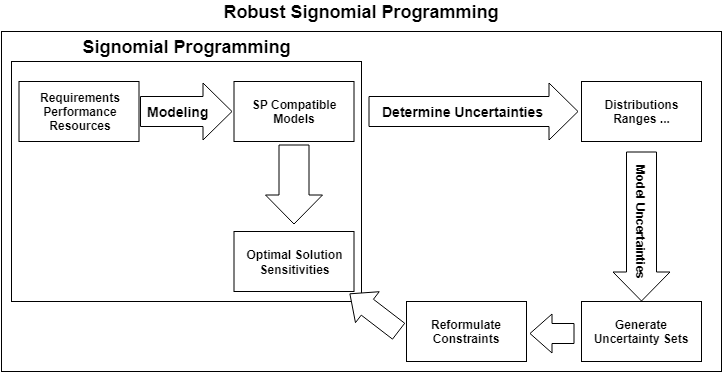
\includegraphics{figures/RSP_Diagram.png}
%	\caption{A block diagram showing the difference between the design process using an SP and an RSP.}
%	\label{block_diag}
%\end{figure}

\begin{figure}
    \begin{center}
    \begin{tikzpicture}[auto, align=center, text width=2.75cm, scale = 0.85]
        \begin{scope}[node distance=2cm]
        \node[block, name=reqs] at (0,0) (reqs) {Requirements \\ Performance \\ Resources};
        \node[block, name=SPmodels] at (6,0) (SPmodels) {SP compatible \\ models};
        \node[block, name=optimum] at (6,-4) (optimum) {Optimal solution \\ Sensitivities};
        \node[block, name=distr] at (14,0) (distr) {Distributions \\ Ranges...};
        \node[block, name=sets] at (14,-4) (sets) {Generate \\ uncertainty sets};
        \node[block, name=reformulate] at (10,-4) (reformulate) {Reformulate constraints};
		\node[name=dummy] at (6, 0.5) (dummy) {};

		    \draw[vecArrow] (reqs) -- node[name=modeling] {\small Modeling} (SPmodels);
			\draw[vecArrow] (SPmodels)to (optimum);
			\draw[vecArrow] (SPmodels) -- node[name=detuncert] {\small Determine uncertainties} (distr);
			\draw[vecArrow] (distr) -- node[name=modeluncert] {\small Model uncertainties} (sets);
 			\draw[vecArrow] (sets) to (reformulate);
			\draw[vecArrow] (reformulate) to (optimum);

		\node[name=SP,label={[xshift=0.0cm, yshift=-3.0cm]\large Signomial Programming},fit=(reqs)(SPmodels)(optimum), draw] {};
		\node[name=RSP,label={[xshift=0.0cm, yshift=0.0cm]\large Robust \\ Signomial \\ Programming \\},
		fit=(SP)(reqs)(SPmodels)(optimum)(distr)(sets)(reformulate)(modeluncert)(detuncert)(modeling)(dummy), draw] {};
		\end{scope}
    \end{tikzpicture}
    \caption{A block diagram showing the difference between the design process using an \gls{sp} and an \gls{rsp}.}
        \label{fig:blockdiag}
\end{center}
\end{figure}


An SP in its \textbf{exponential form} is as follows:

\begin{equation}
    \label{SP_exponential}
\begin{aligned}
	& \min && f_0\left(\vec{x}\right) \\
	& \text{s.t.} && \textstyle{\sum}_{k=1}^{K_i}e^{\vec{a_{ik}}\vec{x} + b_{ik}} - \textstyle{\sum}_{k=1}^{G_i}e^{\vec{c_{ik}}\vec{x} + d_{ik}} \leq 0 \quad \forall i \in 1,...,m\\
\end{aligned}
\end{equation}

Let $\vec{a_{ik}}$ and $\vec{c_{ik}}$ be the $((i-1)\times m + k)^{th}$ rows of the exponents matrices $\mat{A}$ and $\mat{C}$ respectively, and $b_{ik}$ and $d_{ik}$ be the $((i-1)\times m + k)^{th}$ elements of the coefficients vectors $\vec{b}$ and $\vec{d}$ respectively.

The data ($\mat{A}$, $\mat{C}$, $\vec{b}$, $\vec{d}$) is assumed uncertain and living in an uncertainty set $\mathcal{U}$, where $\mathcal{U}$ is parametrized affinely by a perturbation vector $\vec{\zeta}$ as follows:

\begin{equation}
\mathcal{U} = \left\{\left[\mat{A};\mat{C};\vec{b};\vec{d}\right] = \left[\mat{A}^0;\mat{C}^0;\vec{b}^0\;\vec{d}^0 \right] + \textstyle{\sum_{l=1}^{L}\zeta_l\left[\mat{A}^l;\mat{C}^l;\vec{b}^l; \vec{d}^l\right]}\right\}
\label{Data}
\end{equation}
where $\mat{A}^0$, $\mat{C}^0$, $\vec{b}^0$, and $\vec{d}^0$ are the nominal exponents and coefficients, $\left\{\mat{A}^l\right\}_{l=1}^{L}$, $\left\{\mat{C}^l\right\}_{l=1}^{L}$, $\left\{\vec{b}^l\right\}_{l=1}^{L}$, and $\left\{\vec{d}^l\right\}_{l=1}^{L}$ are the basic shifts of the exponents and coefficients, and $\zeta_l$ is the $l^{th}$ component of $\vec{\zeta}$ belonging to a perturbation set $\mathcal{Z} \in \mathbb{R}^L$ such that
\begin{equation}
\mathcal{Z} = \left\{ \vec{\zeta} \in \mathbb{R}^L: \norm{\vec{\zeta}} \leq \Gamma \right\}
\label{perturbation_set}
\end{equation}

As mentioned earlier, there should exist a formulation immune to
uncertainty in the system's data. Accordingly, the robust counterpart
of the uncertain \gls{sp} in \eqref{SP_exponential} is:

\begin{equation}
\begin{aligned}
& \min &&f_0\left(\vec{x}\right)\\
& \text{subject to} &&\max_{\vec{\zeta} \in \mathcal{Z}} \left\{\textstyle{\sum}_{k=1}^{K_i}e^{\vec{a_{ik}}\left(\zeta\right)\vec{x} + b_{ik}\left(\zeta\right)} - \textstyle{\sum}_{k=1}^{G_i}e^{\vec{c_{ik}}\left(\zeta\right)\vec{x} + d_{ik}\left(\zeta\right)}\right\} &&\leq 1 &&\forall i \in 1,...,m\\
\end{aligned}
\label{SP_counterparts_finite}
\end{equation}

The optimization problem in \eqref{SP_counterparts_finite} is intractable using current solvers,
therefore,  a heuristic approach to solving \gls{rsp}s approximately
as a sequential RGP will be presented in the following sections.
As our approach is based on Robust Geometric Programming, a brief review of the subject will follow based on \cite{Saab2018}.
